\documentclass[margin=0mm,tikz]{standalone}
\usetikzlibrary{arrows,arrows.meta,shadows,shapes,shapes.arrows}
\usepackage{graphicx}




\pgfkeys{
/pgf/arrow keys/.cd,
pitch/.code={%
\pgfmathsetmacro\pgfarrowpitch{#1}
\pgfmathsetmacro\pgfarrowsinpitch{abs(sin(\pgfarrowpitch))}
\pgfmathsetmacro\pgfarrowcospitch{abs(cos(\pgfarrowpitch))}
},
}

\pgfdeclarearrow{
name = Cone,
defaults = {       % inherit from Kite
length     = +3.6pt +5.4,
width'     = +0pt +0.5,
line width = +0pt 1 1,
pitch      = +0, % lie on screen
},
cache = false,     % no need cache
setup code = {},   % so no need setup
drawing code = {   % but still need math
% draw the base
\pgfmathsetmacro\pgfarrowhalfwidth{.5\pgfarrowwidth}
\pgfmathsetmacro\pgfarrowhalfwidthsin{\pgfarrowhalfwidth*\pgfarrowsinpitch}
\pgfpathellipse{\pgfpointorigin}{\pgfqpoint{\pgfarrowhalfwidthsin pt}{0pt}}{\pgfqpoint{0pt}{\pgfarrowhalfwidth pt}}
\pgfusepath{fill}
% test if the cone part visible
\pgfmathsetmacro\pgfarrowlengthcos{\pgfarrowlength*\pgfarrowcospitch}
\pgfmathparse{\pgfarrowlengthcos>\pgfarrowhalfwidthsin}
\ifnum\pgfmathresult=1
% it is visible, so draw
\pgfmathsetmacro\pgfarrowlengthtemp{\pgfarrowhalfwidthsin*\pgfarrowhalfwidthsin/\pgfarrowlengthcos}
\pgfmathsetmacro\pgfarrowwidthtemp{\pgfarrowhalfwidth/\pgfarrowlengthcos*sqrt(\pgfarrowlengthcos*\pgfarrowlengthcos-\pgfarrowhalfwidthsin*\pgfarrowhalfwidthsin)}
\pgfpathmoveto{\pgfqpoint{\pgfarrowlengthcos pt}{0pt}}
\pgfpathlineto{\pgfqpoint{\pgfarrowlengthtemp pt}{ \pgfarrowwidthtemp pt}}
\pgfpathlineto{\pgfqpoint{\pgfarrowlengthtemp pt}{-\pgfarrowwidthtemp pt}}
\pgfpathclose
\pgfusepath{fill}
\fi
\pgfpathmoveto{\pgfpointorigin}
}
}

\definecolor{As}{RGB}{255,255,0}
\definecolor{Al}{RGB}{173,216,230}
\definecolor{Ga}{RGB}{0,128,150}

\begin{document}
	\begin{tikzpicture}[remember picture]
		\useasboundingbox (-80mm,7mm) rectangle (120mm,150mm);
		\draw[left color=black!50, right color=black!50, middle color=white,fill opacity=1,line width=0.3mm] (-60mm,70mm)--(60mm,70mm)--(40mm,97mm)--(-40mm,97mm)--cycle;
		%\draw (-50mm,70mm)--(-45mm,20mm);
		%\draw (45mm,70mm)--(45mm,30mm);
		\draw [black,-,left color=black!35, right color=black!35, middle color=white,line width=0.4mm] plot [smooth,tension=1] coordinates { 
		(-60mm,20mm) (-15mm,10mm) (20mm,35mm) (60mm,30mm)}--(60mm,70mm)--(-60mm,70mm)--cycle;
		
		\draw[-{Cone      },line width=2mm](0,8.5,0)--(6.5,7,0);
		\draw[-{Cone      },line width=2mm](0,8.5,0)--(-6.5,7,0);
		\draw[-{Cone [pitch=0]     },line width=2mm](0,8.5,0)--(-2.7,8.5,-7);
		
		\node[scale=3] at (15mm,115mm){$\left[001\right]$};
		\node[scale=3] at (-35mm,60mm){$\left[1\overline{1}0\right]$};
		\node[scale=3] at (35mm,60mm){$\left[110\right]$};
		\node[scale=4,font=\bf] at (-40mm,30mm){\textcolor{Ga}{Ga}\textcolor{As}{As}};
		
		\node[anchor=center,yshift=0mm](str) at (80mm,115mm){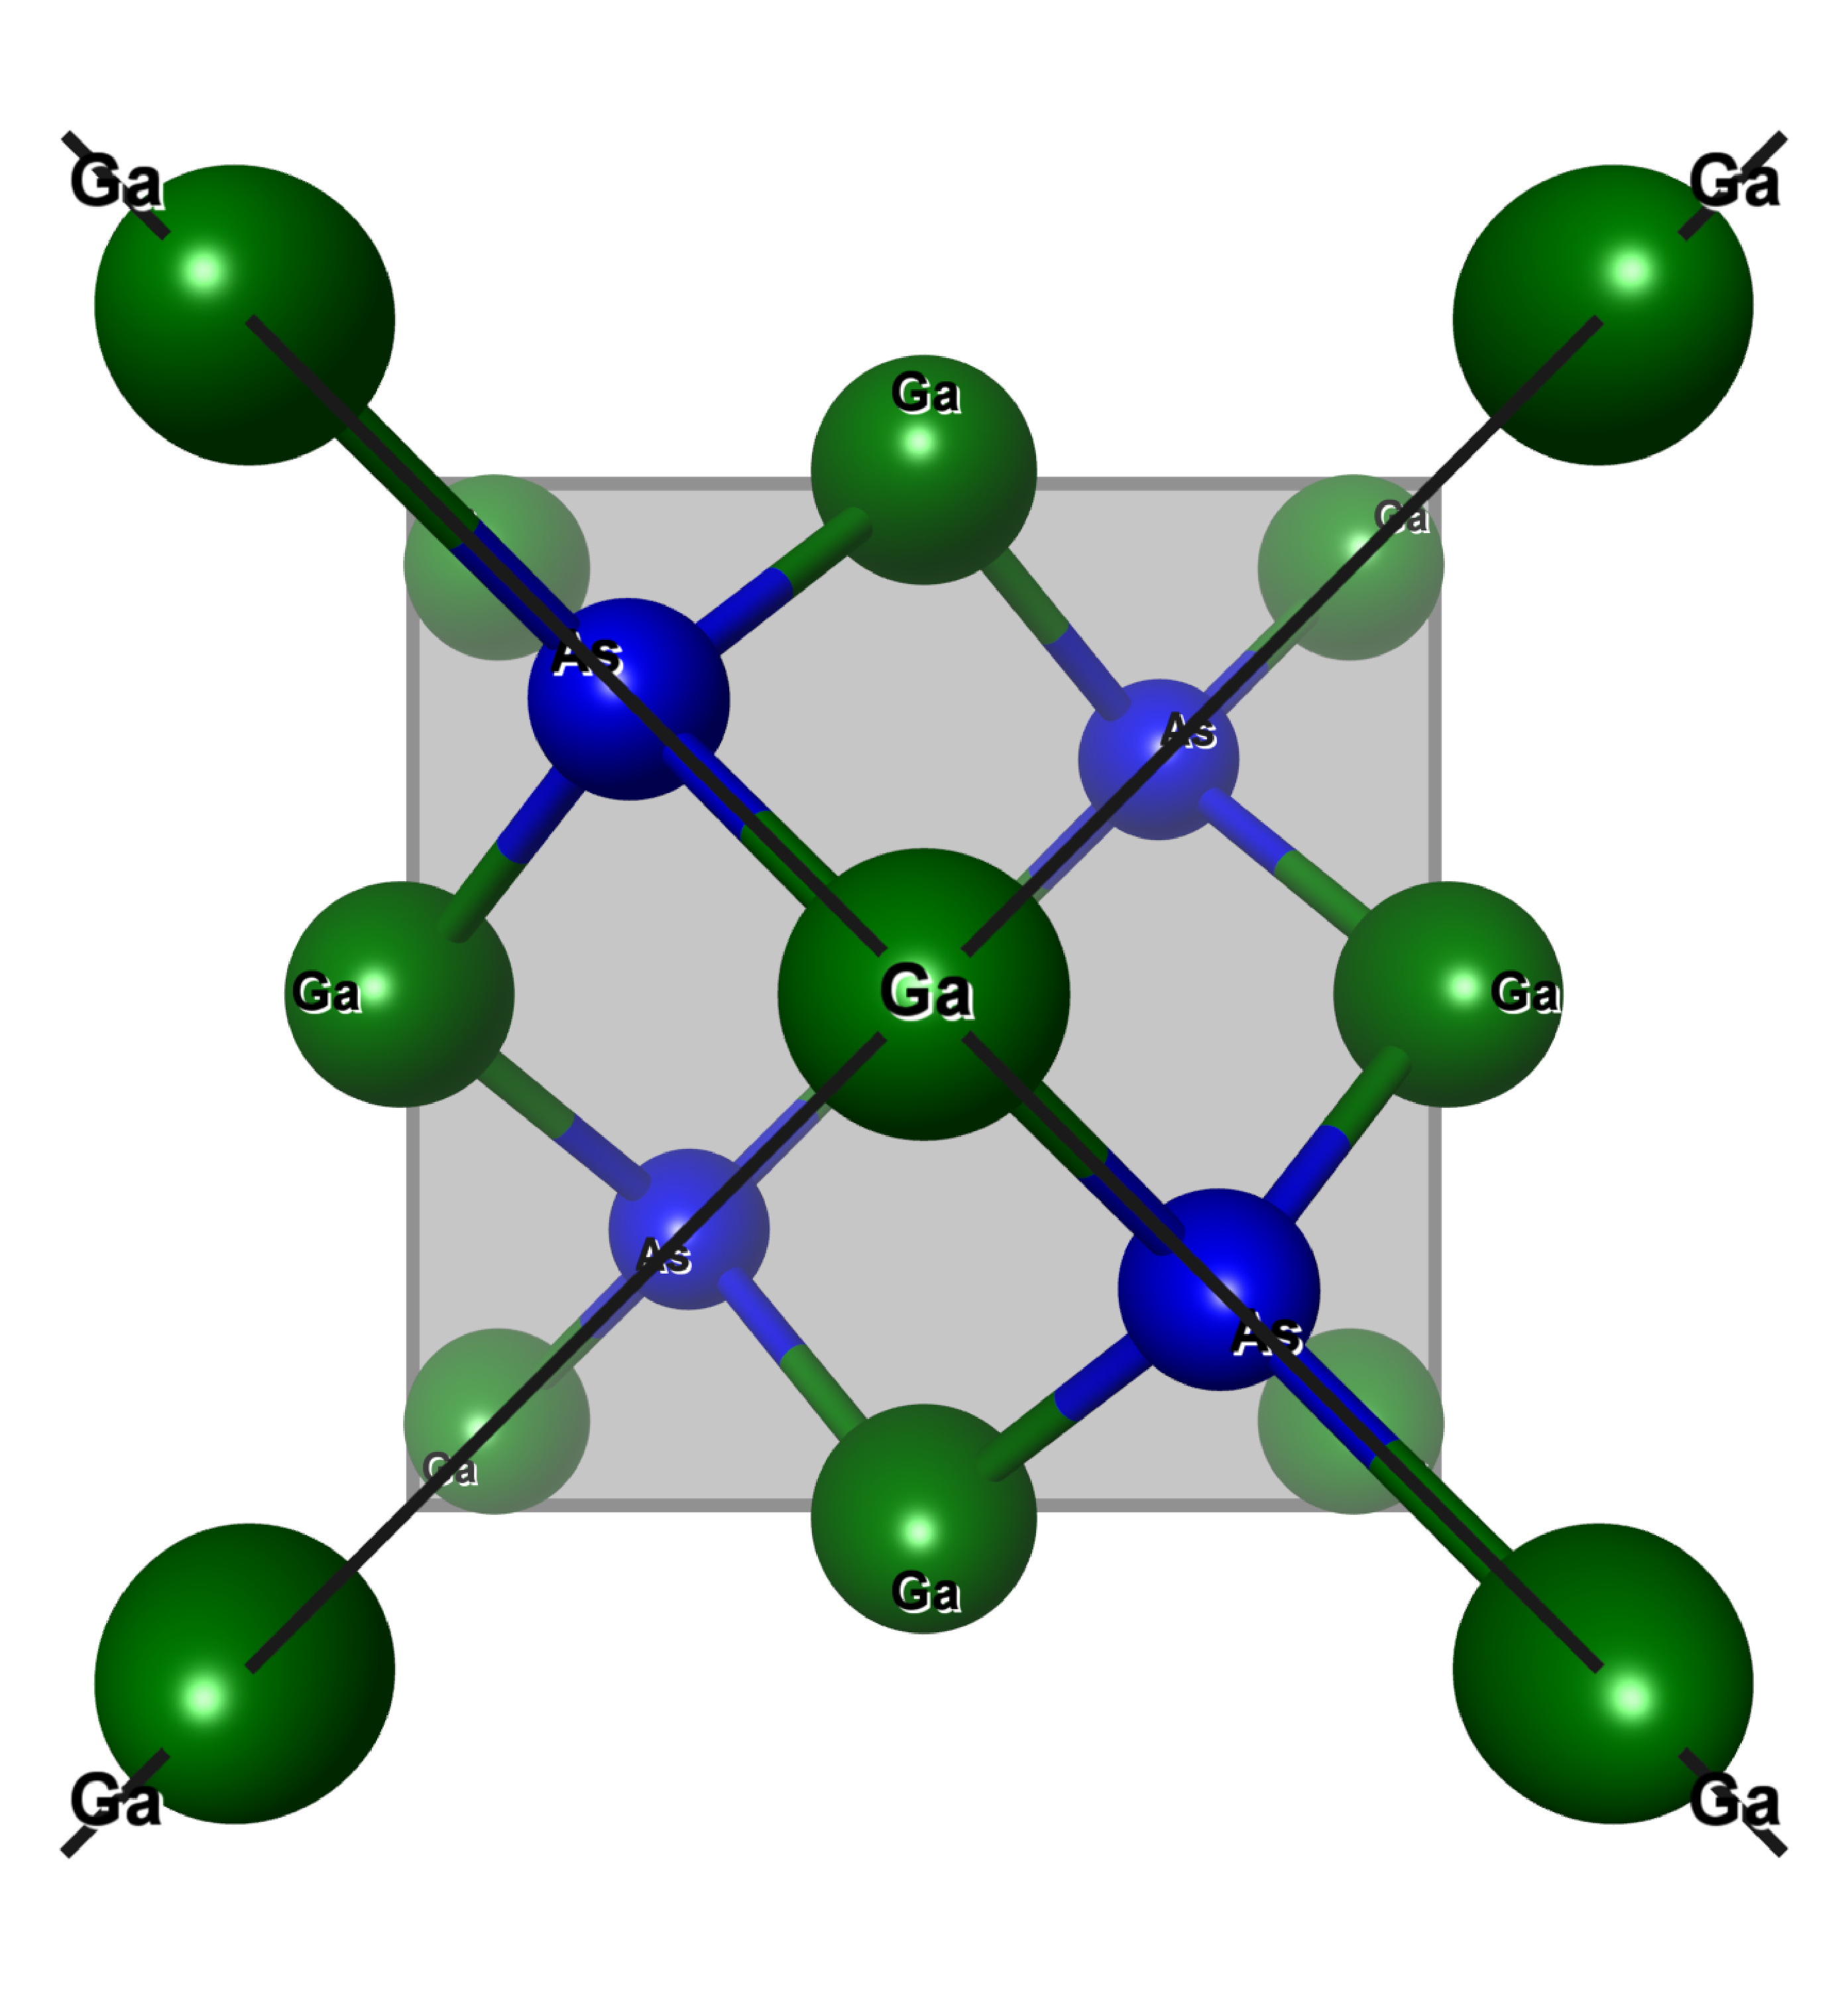
\includegraphics[width=0.6\linewidth]{/media/labfiles/ruco/phd-ssp/scripts/structures/GaAs.pdf}};


\shade [ball color=Ga] ([xshift=-2cm,yshift=-1cm]str.south east) circle (0.5) node[label=right:{\huge\, \textbf{Ga}},font=\bf](Ga) { } ;
%\shade [ball color=Al] (-3.3,6.5) circle (0.3) node[label=right:{\Large\, Al}] { } ;
\shade [ball color=As] ([xshift=0cm,yshift=-1cm]Ga.south) circle (0.5) node[label=right:{\huge\, \textbf{As}},font=\bf] { };	
	\end{tikzpicture}
\end{document}